\documentclass[aspectratio=169,11pt]{beamer}

\usepackage[T1]{fontenc}
\usepackage[utf8]{inputenc}
\usepackage{lmodern}
\usepackage{microtype}
\usepackage{graphicx}
\usepackage{booktabs}
\usepackage{tabularx}
\usepackage{tikz}
\usetikzlibrary{arrows.meta,positioning,shapes.geometric}

% IITG and Custom Colors
\definecolor{iitgblue}{HTML}{163A63}
\definecolor{srfdgreen}{HTML}{3A7D44}
\definecolor{srfdorange}{HTML}{D97706}
\definecolor{softblue}{HTML}{EAF2F8}
\definecolor{softgreen}{HTML}{EAF6EC}
\definecolor{softorange}{HTML}{FFF4E5}
\definecolor{softgray}{HTML}{F3F4F6}

% Beamer Theme Customization
\setbeamertemplate{navigation symbols}{}
\setbeamercolor{structure}{fg=iitgblue}
\setbeamercolor{frametitle}{bg=iitgblue,fg=white}
\setbeamercolor{title}{fg=iitgblue}
\setbeamercolor{itemize item}{fg=srfdgreen}
\setbeamercolor{itemize subitem}{fg=srfdorange}
\setbeamertemplate{footline}[frame number]

% TikZ Styles
\tikzset{
  state/.style={circle,draw=iitgblue,very thick,minimum size=13mm,fill=softblue,font=\bfseries},
  trans/.style={-{Stealth[length=2.5mm]},thick,iitgblue},
  block/.style={rounded corners,draw=iitgblue,thick,fill=softblue,minimum width=24mm,minimum height=10mm,align=center},
  srfdblock/.style={rounded corners,draw=srfdgreen,very thick,fill=softgreen,minimum width=28mm,minimum height=11mm,align=center},
  decision/.style={diamond,aspect=2,draw=srfdorange,thick,fill=softorange,align=center,inner sep=1.5pt},
  flow/.style={-{Stealth[length=2.2mm]},thick}
}

\title{Reducing Off-Chip Miss Penalty by Exploiting Underutilised On-Chip Router Buffers}
\subtitle{Implementation and Evaluation in gem5}
\author{Pranjal (230101077) \and Pratyush (230101079)}
\institute{Department of Computer Science and Engineering\\Indian Institute of Technology Guwahati}
\date{Mid-Term Evaluation \\ Academic Year 2026--2027}

\begin{document}

\begin{frame}
  \titlepage
\end{frame}

\begin{frame}{Motivation \& Problem Statement}
  \begin{itemize}
    \item \textbf{High Off-Chip Penalty:} LLC misses force requests to travel through the NoC to off-chip memory, incurring massive latency.
    \item \textbf{Underutilised Resources:} NoC virtual channel (VC) buffers are frequently idle outside of short congestion bursts.
    \item \textbf{Objective:} Implement the \emph{Store, Reply, Forward and Drop} (SRFD) mechanism in gem5 to temporarily retain evicted blocks in local routers, providing fast local replies without violating MOESI coherence.
  \end{itemize}
\end{frame}

\begin{frame}{Identifying the Problem: Key Metrics}
  \begin{columns}
    \begin{column}{0.45\textwidth}
      \begin{itemize}
        \item \textbf{LLC Miss Penalty:} Time from issuing an off-chip GETS/GETX at L2 until the response data reaches L2 (about 151--167 Ruby cycles in the completed baselines).
        \item \textbf{VC Availability:} The fraction of execution cycles where NoC virtual channels remain unused.
        \item \textbf{Re-reference Time:} The duration from eviction to a future request for the same LLC block; this is the metric plotted in thousands of cycles.
      \end{itemize}
    \end{column}
    \begin{column}{0.5\textwidth}
      \centering
      % Replace with your VC availability and Re-reference time charts
      \fbox{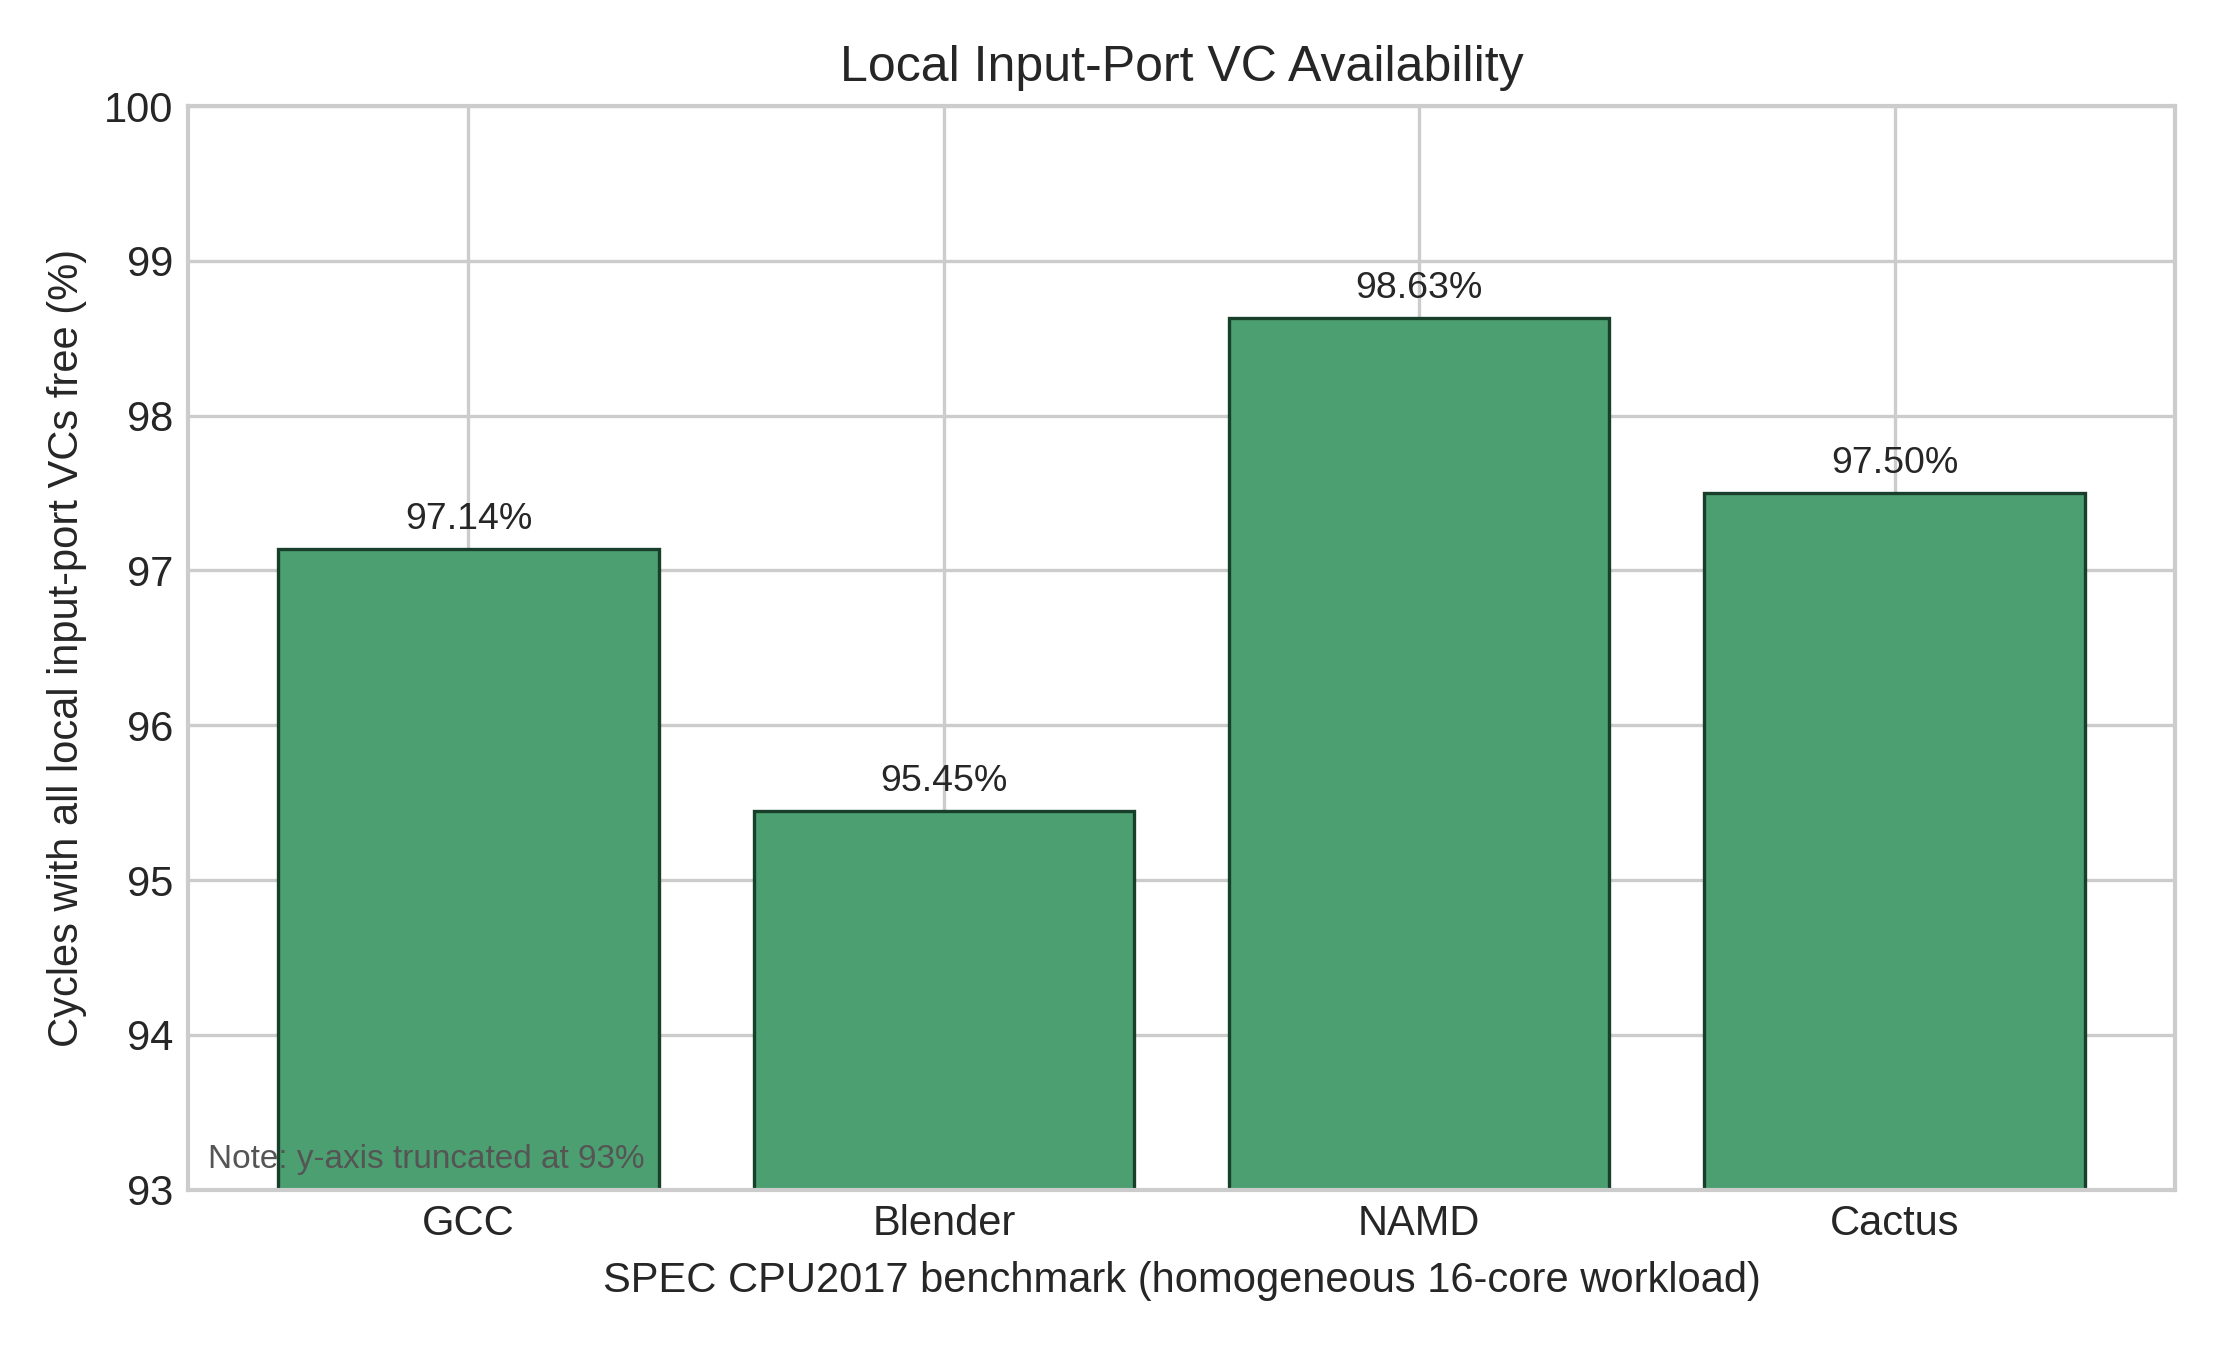
\includegraphics[width=0.9\linewidth,height=3cm,keepaspectratio]{vc_availability.png}}

      \vspace{0.2cm}

      \fbox{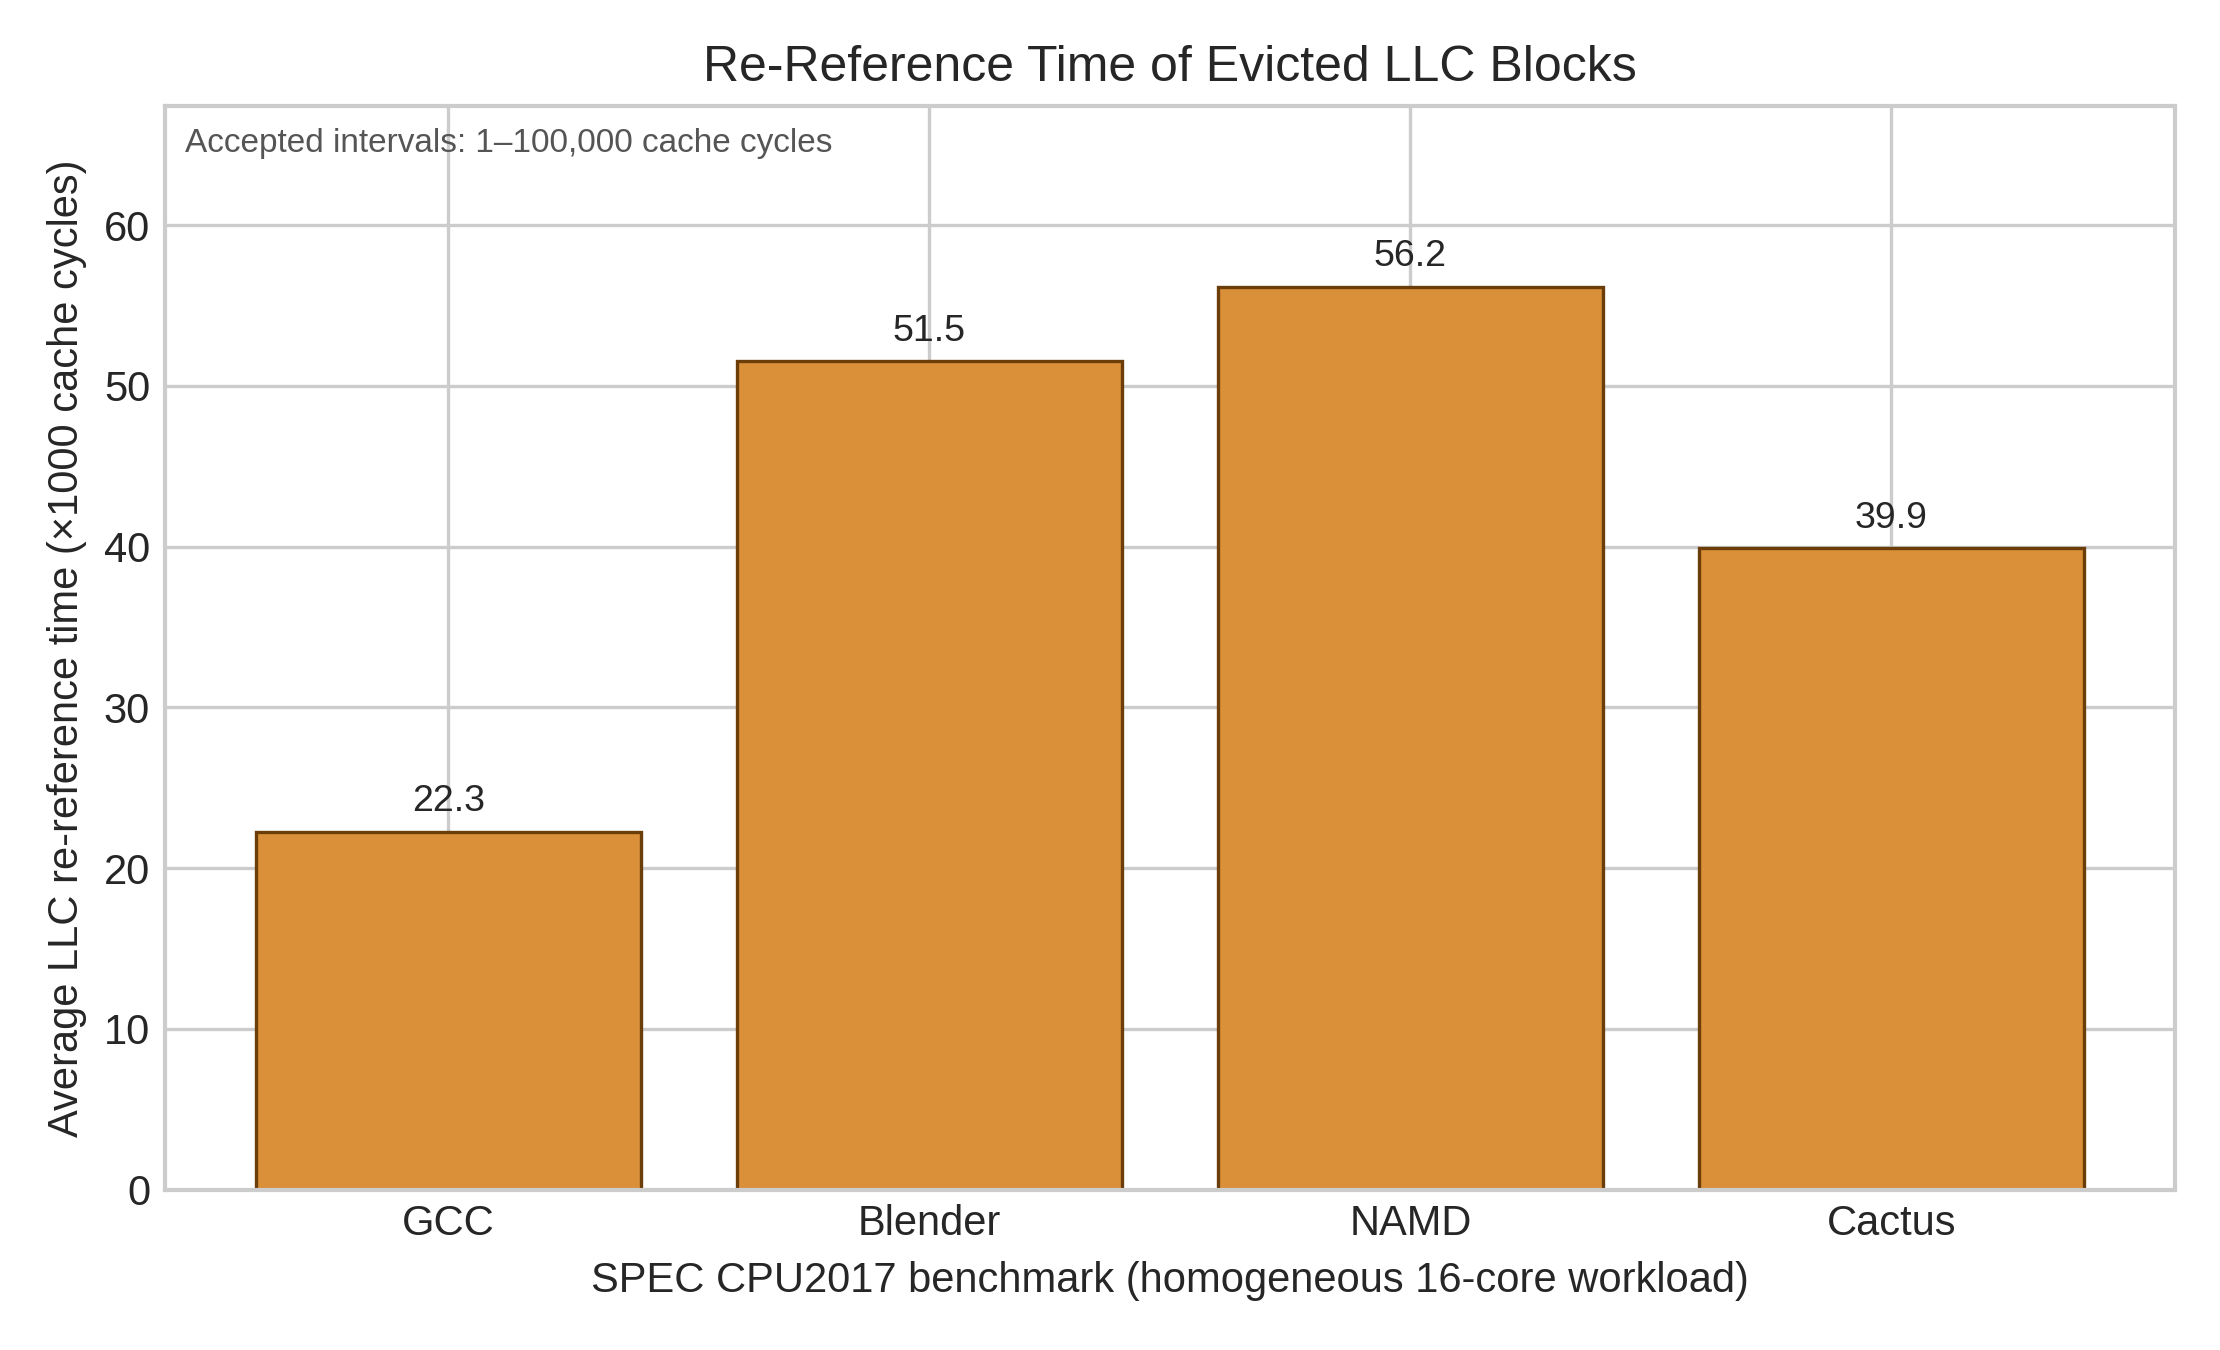
\includegraphics[width=0.9\linewidth,height=3cm,keepaspectratio]{re_reference_cycles.png}}

      \scriptsize ``$\times 1000$ cycles'' applies to re-reference time, not LLC miss penalty.
    \end{column}
  \end{columns}
\end{frame}

\begin{frame}{Proposed Solution: The SRFD Mechanism}
  \begin{itemize}
    \item \textbf{Store:} Retain an eligible eviction-data packet in the local router.
    \item \textbf{Reply:} Match a later request and return the retained data locally, avoiding memory round-trips.
    \item \textbf{Forward:} Release dirty retained data toward memory when router buffer pressure requires it.
    \item \textbf{Drop:} Discard clean retained data when pressure requires the VC (memory already has a valid copy).
  \end{itemize}
\end{frame}

\begin{frame}{Meaning of the SRFD Counters}
  \footnotesize
  \begin{columns}[T]
    \begin{column}{0.49\textwidth}
      \textbf{Eviction-data lifecycle}
      \begin{itemize}
        \item \textbf{Offered:} marked clean/dirty eviction reaches the local router.
        \item \textbf{Stored:} its complete packet is retained in one data VC.
        \item \textbf{Clean dropped:} clean copy is discarded under pressure or on a GETX conflict.
        \item \textbf{Dirty forwarded:} dirty copy resumes its path to memory under pressure.
      \end{itemize}
    \end{column}
    \begin{column}{0.49\textwidth}
      \textbf{Request lifecycle}
      \begin{itemize}
        \item \textbf{Eligible lookup:} marked off-chip GETS/GETX searches the local stored entries.
        \item \textbf{Clean hit:} GETS receives shared data locally.
        \item \textbf{Dirty hit:} GETS/GETX receives data locally and inherits writeback responsibility.
        \item \textbf{Avoided request:} local reply avoids the ordinary memory data return.
      \end{itemize}
    \end{column}
  \end{columns}
  \vspace{0.1cm}
  \centering
  \fbox{\parbox{0.88\linewidth}{\centering
  $\text{hits}=\text{clean hits}+\text{dirty hits}$\quad and\quad
  $\text{hit rate}=\text{hits}/(\text{GETS lookups}+\text{GETX lookups})$}}
\end{frame}

\begin{frame}{SRFD Mode Names and Pressure Policies}
  \small
  \begin{columns}[T]
    \begin{column}{0.47\textwidth}
      \textbf{What may be stored?}
      \begin{itemize}
        \item \textbf{DB: Dirty Blocks only.} A released block must be forwarded to memory.
        \item \textbf{CB+DB: Clean and Dirty Blocks.} A released clean block may be dropped; dirty data is forwarded.
        \item \textbf{Baseline:} no router storage or local matching.
      \end{itemize}
    \end{column}
    \begin{column}{0.51\textwidth}
      \textbf{When is the oldest entry released?}
      \begin{itemize}
        \item \textbf{Defensive:} VC allocation fails and at least one complete stored victim exists.
        \item \textbf{Aggressive:} release only when all six VCs of the relevant vnet contain complete SRFD packets.
      \end{itemize}
    \end{column}
  \end{columns}
  \vspace{0.15cm}
  \begin{block}{Examples}
    \centering
    \texttt{db-defensive} = dirty only + early release\qquad
    \texttt{cbdb-aggressive} = clean and dirty + retain until full
  \end{block}
\end{frame}


\begin{frame}{4$\times$4 Ruby Network Topology}
  \centering
  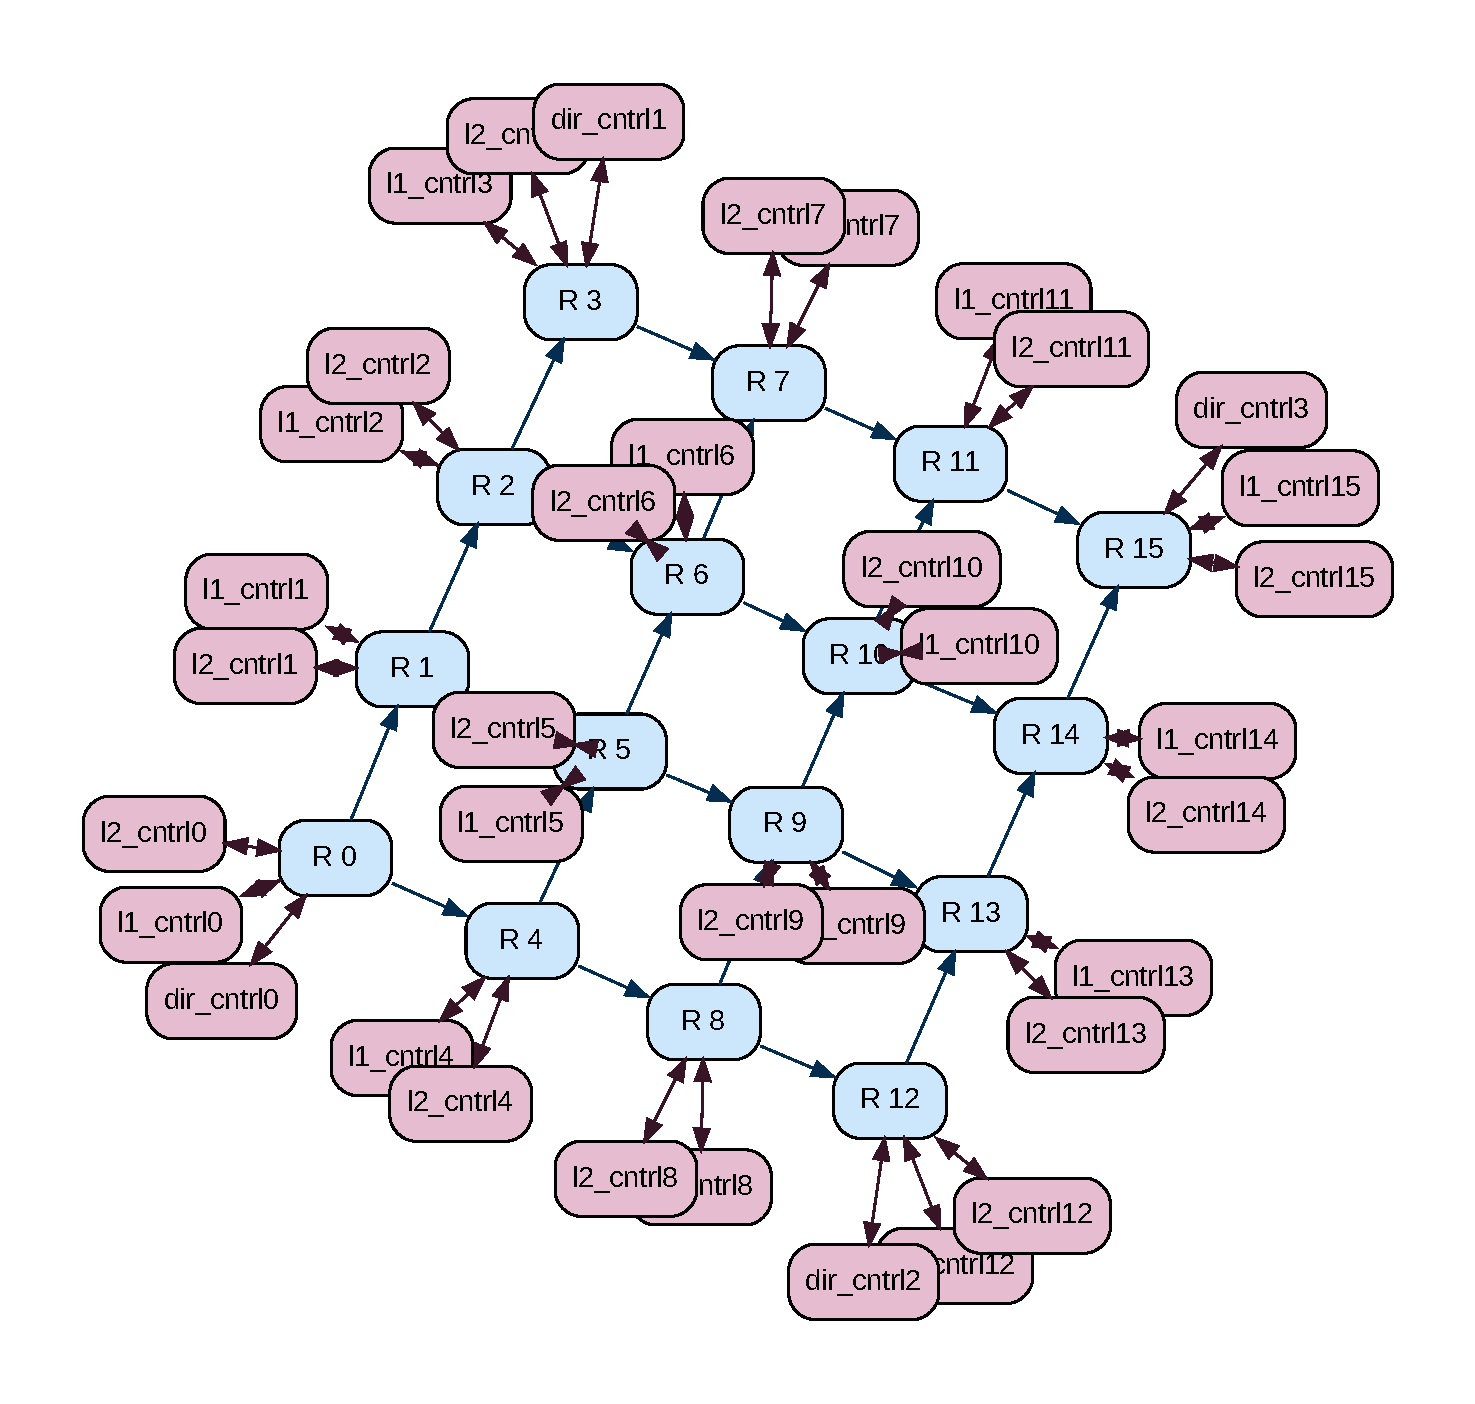
\includegraphics[width=0.94\linewidth,height=0.72\textheight,keepaspectratio]{config.system.ruby.dot.pdf}

  \vspace{0.1cm}
  \small 16 routers in a 4$\times$4 mesh, with directory controllers at
  routers 0, 3, 12, and 15. Each core has a private L1 controller and an
  associated shared LLC bank; the network uses six VCs per vnet.
\end{frame}


\begin{frame}{SRFD Transient States and Transitions}
  \textbf{New SRFD Transient States}
  \vspace{0.1cm}

  \resizebox{\linewidth}{!}{
  \begin{tabular}{@{}llllp{7.5cm}l@{}}
    \toprule
    \textbf{Category} & \textbf{New state} & \textbf{Entered from} & \textbf{Meaning} & \textbf{Final state} \\
    \midrule
    \textcolor{srfdgreen}{\rule{1.2ex}{1.2ex}} New SRFD state & \texttt{IGS\_SRFD} & \texttt{IGS} & A clean block stored in the local router has satisfied GETS. Data was sent to the requesting L1, and the controller is waiting for Unblock. & \texttt{ILS} \\
    \textcolor{srfdgreen}{\rule{1.2ex}{1.2ex}} New SRFD state & \texttt{IGMOU\_SRFD} & \texttt{IGS} or \texttt{IGM} & A dirty stored block has satisfied GETS or GETX. Data was sent with exclusive/modified responsibility, and the controller is waiting for Exclusive\_Unblock. & \texttt{ILX} \\
    \bottomrule
  \end{tabular}
  }

  \vspace{0.5cm}
  \textbf{SRFD State Transitions}
  \vspace{0.1cm}

  \resizebox{\linewidth}{!}{
  \begin{tabular}{@{}llll@{}}
    \toprule
    \textbf{Request} & \textbf{Router match} & \textbf{New transition} & \textbf{Result} \\
    \midrule
    GETS & Clean stored block & \texttt{IGS} $\rightarrow$ \texttt{IGS\_SRFD} $\rightarrow$ \texttt{ILS} & L1 receives shared data. \\
    GETS & Dirty stored block & \texttt{IGS} $\rightarrow$ \texttt{IGMOU\_SRFD} $\rightarrow$ \texttt{ILX} & L1 receives exclusive data and inherits writeback responsibility. \\
    GETX & Dirty stored block & \texttt{IGM} $\rightarrow$ \texttt{IGMOU\_SRFD} $\rightarrow$ \texttt{ILX} & L1 receives exclusive/modified data. \\
    GETX & Clean stored block & No new L2 transition & Router drops the clean stored block; GETX continues to memory. \\
    GETS/GETX & No match & Existing controller transition & Request proceeds through the directory/memory hierarchy normally. \\
    \bottomrule
  \end{tabular}
  }
\end{frame}
\begin{frame}{Router-Side Storage \& Pressure Policies}
  \centering
  % Replace with the image you generate from the standalone TikZ code below
  \includegraphics[width=0.9\linewidth,height=0.75\textheight,keepaspectratio]{Router.png}
\end{frame}

\begin{frame}{Implementation Progress}
  \textbf{Completed in gem5:}
  \begin{itemize}
    \item Runtime-selectable baseline and SRFD operating modes.
    \item SRFD metadata propagation via Ruby messages and Garnet flits.
    \item Router-buffer storage and off-chip GETS/GETX address matching.
    \item Clean and dirty local-reply paths in the L2 controller.
    \item Directory synchronisation and coherence recovery using \texttt{CAN\_PUT}.
    \item Instrumentation for VC availability, local replies, and network pressure.
  \end{itemize}
\end{frame}

\begin{frame}{4$\times$4 Results: LLC Miss Penalty}
  \centering
  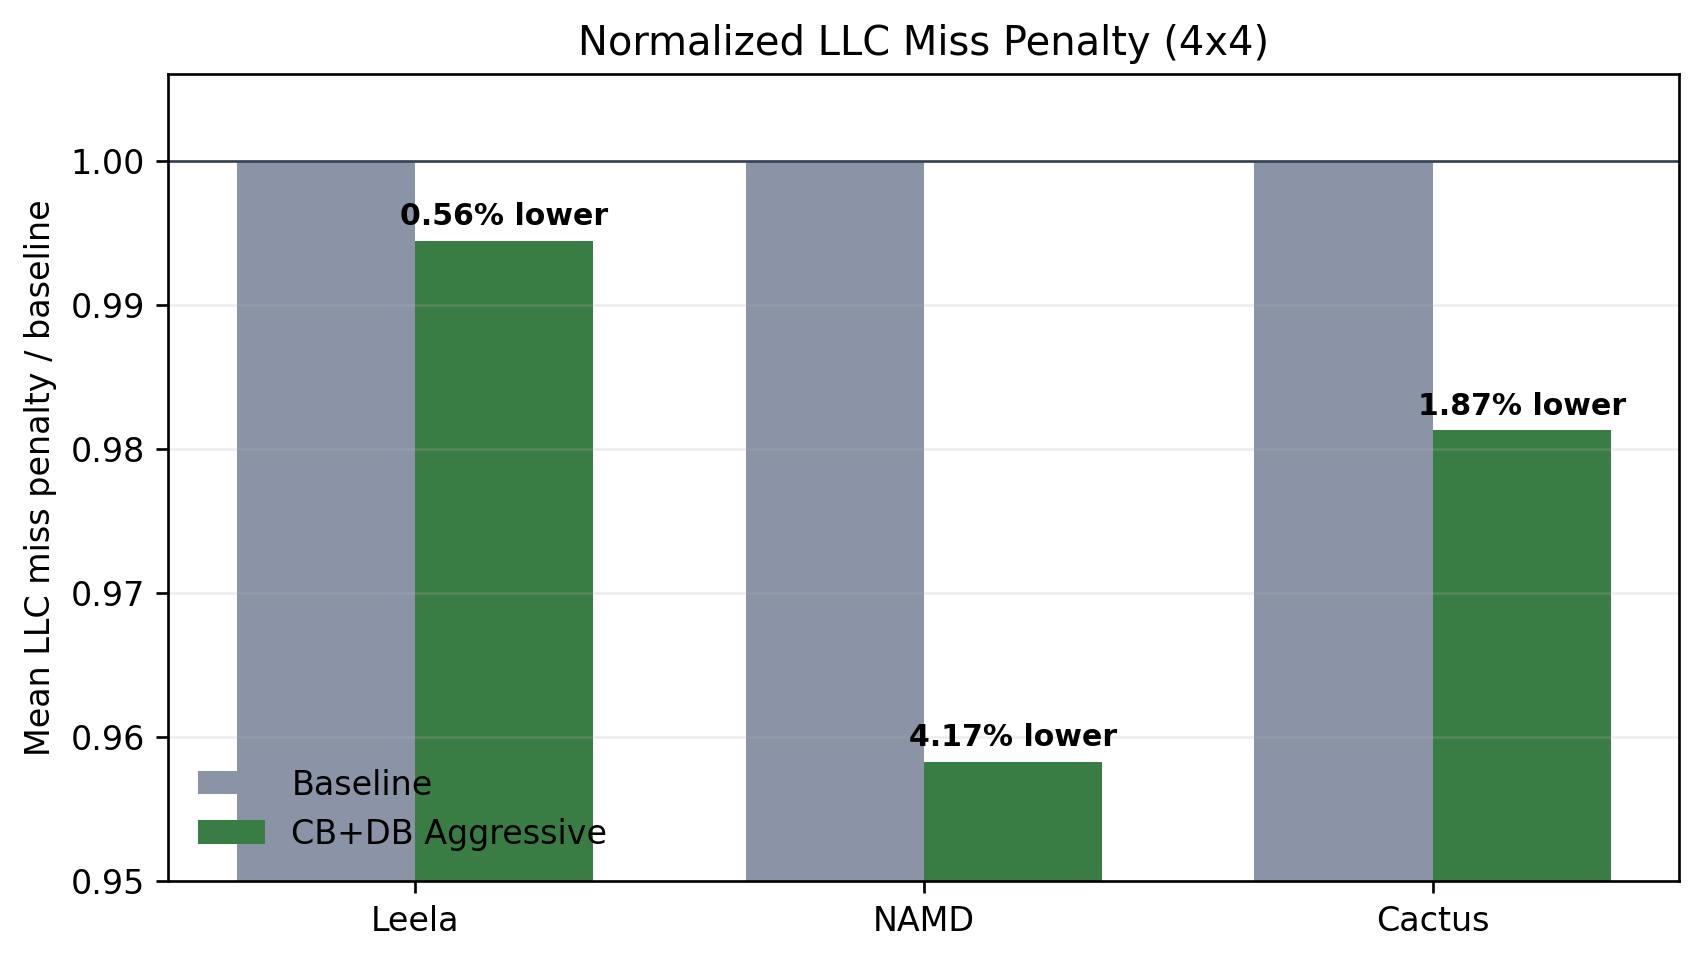
\includegraphics[width=0.83\linewidth,height=0.69\textheight,keepaspectratio]{srfd_4x4_llc_penalty.png}

  \vspace{-0.1cm}
  \small CB+DB Aggressive reduced mean LLC miss penalty for all three completed
  workloads: Leela 0.56\%, NAMD 4.17\%, and Cactus 1.87\%. NAMD is the
  checkpointed computation-only 20M-instruction/core ROI. The metric is in Ruby
  cycles, from off-chip GETS/GETX issue at L2 until response data reaches L2.
\end{frame}

\begin{frame}{4$\times$4 Results: Router-Buffer Usefulness}
  \begin{columns}
    \begin{column}{0.5\textwidth}
      \centering
      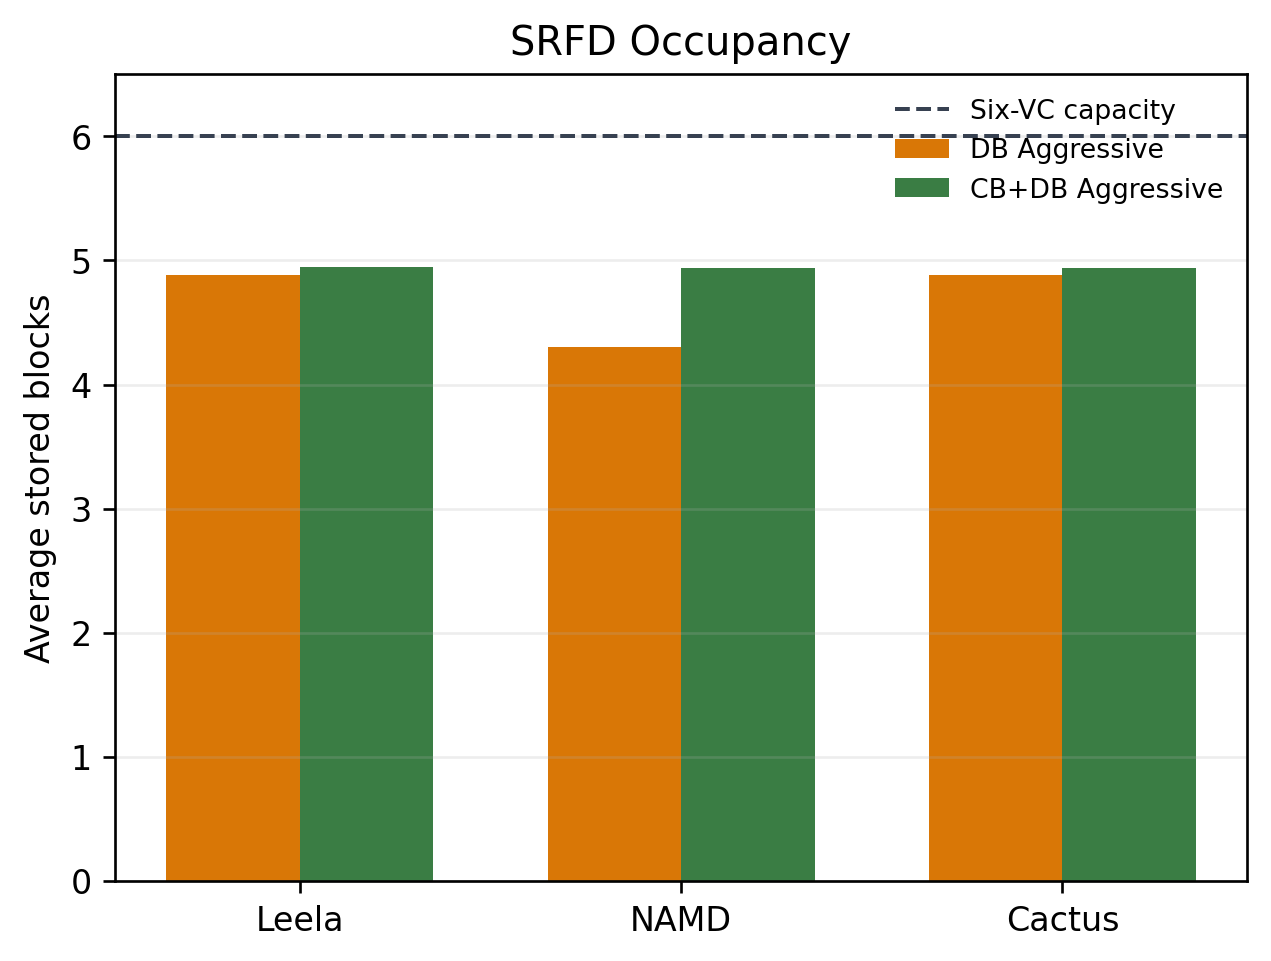
\includegraphics[width=\linewidth,height=0.58\textheight,keepaspectratio]{srfd_4x4_occupancy.png}
    \end{column}
    \begin{column}{0.5\textwidth}
      \centering
      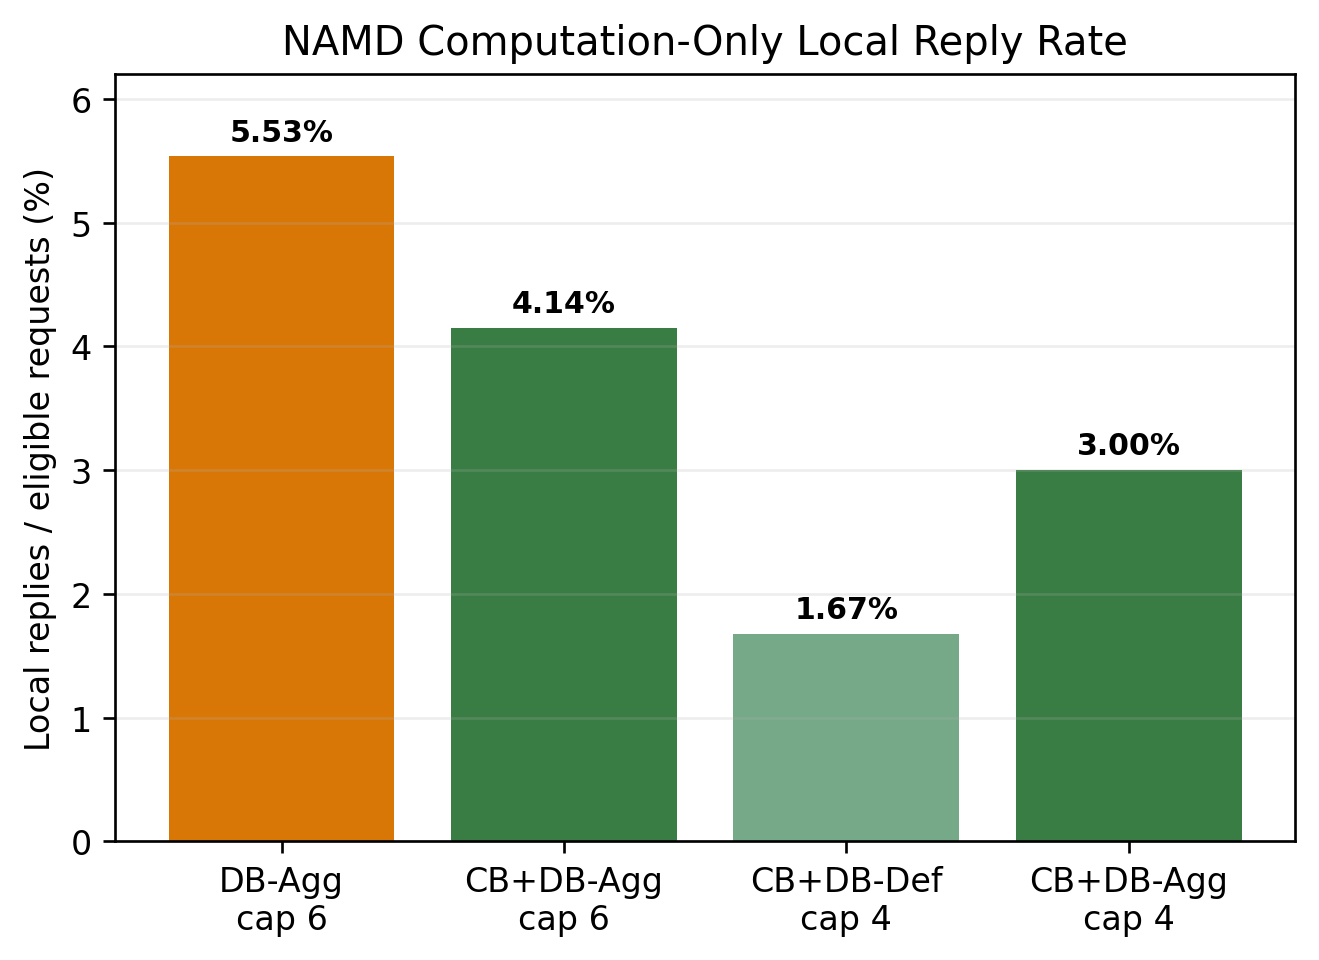
\includegraphics[width=\linewidth,height=0.58\textheight,keepaspectratio]{srfd_4x4_hit_rate_trend.png}
    \end{column}
  \end{columns}
  \small
  \begin{itemize}
    \item In the NAMD computation ROI, cap-6 DB-Aggressive and CB+DB-Aggressive average \textbf{4.30} and \textbf{4.94} retained blocks per L2-facing input.
    \item NAMD local-reply rate reaches 5.53\% for DB-Aggressive and 4.14\% for CB+DB-Aggressive; reserving two VC slots lowers CB+DB rates to 1.67--3.00\%.
  \end{itemize}
\end{frame}

\begin{frame}{NAMD: Ruby Buffer Stall Comparison}
  \centering
  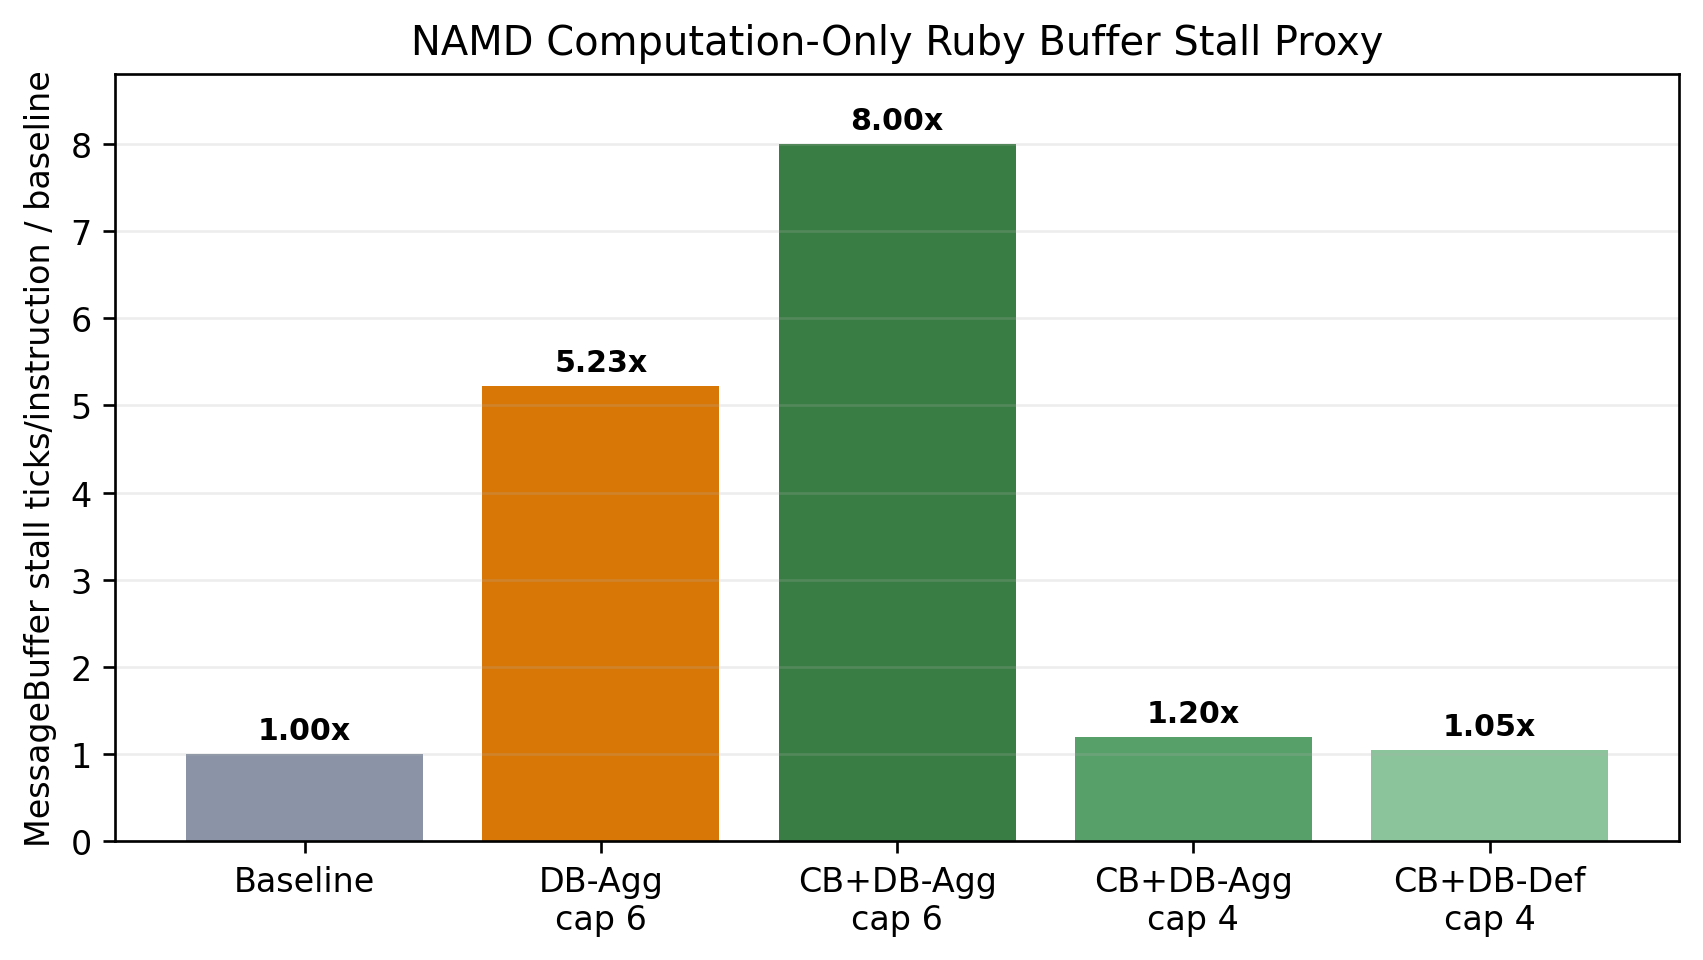
\includegraphics[width=0.9\linewidth,height=0.59\textheight,keepaspectratio]{namd_message_buffer_stall.png}

  \small
  \begin{itemize}
    \item The value sums Ruby \texttt{MessageBuffer::m\_stall\_time}, divides by simulated instructions, and normalizes to the computation-only baseline.
    \item Cap 6 raises this queue-residence proxy to 5.23$\times$ (DB) and 8.00$\times$ (CB+DB); cap 4 limits it to 1.20$\times$ aggressive and 1.05$\times$ defensive.
    \item A retained block's own router residence is measured separately. It affects this proxy indirectly when occupied VCs delay source-message injection.
  \end{itemize}
\end{frame}

\begin{frame}{NAMD: Retained-Block Timing}
  \small
  \centering
  \begin{tabular}{@{}lrr@{}}
    \toprule
    \textbf{Policy} & \textbf{Mean residence} & \textbf{Cycles/local reply} \\
    \midrule
    DB-Aggressive, cap 6 & 36,344.75 & 1,316.76 \\
    CB+DB-Aggressive, cap 6 & 7,940.49 & 1,698.74 \\
    CB+DB-Aggressive, cap 4 & 5,552.56 & 2,278.65 \\
    CB+DB-Defensive, cap 4 & 2,142.73 & 4,150.07 \\
    \bottomrule
  \end{tabular}

  \vspace{0.35cm}
  \begin{block}{Interpretation}
    Mean residence is sample-weighted over retired retained packets and mixes
    local hits, pressure forwarding, and clean drops. Cycles/local reply is ROI
    cycles divided by all local replies across 16 cores; current counters do not
    expose store-to-hit-only latency or the hit inter-arrival distribution.
  \end{block}
\end{frame}

\begin{frame}{NAMD: Retention Benefit and Pressure Overhead}
  \small
  \textbf{Original CB+DB-Aggressive policy:} all six data VCs available for
  retention; computation-only 20M-instruction/core ROI.
  \vspace{0.15cm}

  \centering
  \begin{tabular}{@{}lr@{}}
    \toprule
    \textbf{Metric} & \textbf{Measured value} \\
    \midrule
    Clean hits & 5,429 (2.144\%) \\
    Dirty hits & 5,067 (2.001\%) \\
    Combined hit rate & 4.145\% \\
    Clean + dirty blocks stored & 177,336 \\
    Mean retained occupancy & 4.94 of 6 VCs \\
    Pressure attempts & 46,215,821 \\
    Successful pressure releases & 166,803 \\
    Aggregate IPC & 18.905 ($-3.24\%$ vs baseline) \\
    Mean LLC miss penalty & 159.59 cycles \\
    \bottomrule
  \end{tabular}

  \vspace{0.25cm}
  \begin{alertblock}{Observed trade-off}
    Local replies reduce the baseline LLC penalty of 166.54 cycles, but the
    retained packets consume most data VCs. Repeated failed VC allocation
    checks indicate substantial injection backpressure, and total IPC decreases.
  \end{alertblock}
\end{frame}

\begin{frame}{NAMD: Reducing SRFD Retention Overhead}
  \small
  \textbf{Computation-only ROI:} 16 O3 cores, 4$\times$4 mesh, six VCs per
  vnet, 20M minimum measured instructions per core.
  \vspace{0.15cm}

  \centering
  \resizebox{\linewidth}{!}{%
  \begin{tabular}{@{}lrrr@{}}
    \toprule
    \textbf{Metric} & \textbf{Baseline} & \textbf{Cap 6} & \textbf{Cap 4} \\
    \midrule
    Retained blocks per L2-facing input & 0 & 6 & 4 \\
    Combined clean+dirty hit rate & --- & 4.145\% & 3.004\% \\
    NI allocation checks (attempts) & 0 & 46,215,821 & 2,117,460 \\
    Successful block releases & 0 & 166,803 & 149,162 \\
    Aggregate IPC & 19.537 & 18.905 & 19.628 \\
    IPC change vs baseline & --- & $-3.24\%$ & $+0.46\%$ \\
    Mean LLC miss penalty (cycles) & 166.54 & 159.59 & 162.19 \\
    \bottomrule
  \end{tabular}}

  \vspace{0.3cm}
  \begin{block}{Headroom trade-off}
    Reserving two VCs reduces maximum SRFD retention from 96 to 64 blocks
    across the 16 L2-facing inputs. Hit rate falls by 1.14 percentage points,
    but pressure attempts fall by 95.4\%; the previous 3.24\% IPC loss becomes
    a 0.46\% IPC gain over baseline.
  \end{block}
\end{frame}

\begin{frame}{Observations from the Mid-Evaluation Runs}
  \textbf{Completed configuration:} 16 cores, 4$\times$4 MeshDirCorners\_XY,
  and six VCs per vnet. The updated NAMD result uses O3 CPUs and its
  checkpointed computation-only 20M-instruction/core ROI.
  \begin{itemize}
    \item NAMD CB+DB-Aggressive averages 4.94 complete retained packets in the six eligible data VCs; DB-Aggressive averages 4.30.
    \item Local clean and dirty replies occur without an off-chip data return, demonstrating the complete Store--Reply--\texttt{CAN\_PUT} path.
    \item Cactus provides the strongest current result: 1,025 local replies and a 1.87\% lower mean LLC miss penalty with CB+DB Aggressive.
    \item The measured local-reply rate remains workload-dependent; longer runs and the paper-scale topology are required for final performance conclusions.
  \end{itemize}

  \vspace{0.15cm}
  \begin{alertblock}{Interpretation}
    The mid-evaluation evidence establishes functional SRFD operation and measurable LLC-latency reduction on the completed 4$\times$4 experiments. It is not yet a reproduction of the paper's 64-core OoO evaluation.
  \end{alertblock}
\end{frame}

\begin{frame}{Validation Status}
  \textbf{Current Validation:}
  \begin{itemize}
    \item Directed testing of clean/dirty GETS/GETX and clean-GETX conflicts.
    \item Verification of \texttt{CAN\_PUT} accounting and stored packet lifetimes.
    \item Completed 4$\times$4 measurements for Leela, NAMD, and Cactus across baseline, DB, and CB+DB policies.
  \end{itemize}

  \vspace{0.25cm}
  \textbf{Next Evaluation Steps:}
  \begin{itemize}
    \item Complete the 64-core homogeneous workload evaluations.
    \item Analyze system IPC, LLC miss penalty reduction, and wait cycles.
  \end{itemize}
\end{frame}

\begin{frame}{Future Work: Balancing Hits and NoC Headroom}
  \small
  \begin{alertblock}{Updated NAMD result}
    The original cap-six policy reaches a 4.145\% hit rate but loses 3.24\%
    IPC. Reserving two VCs lowers the hit rate to 3.004\%, reduces pressure
    attempts by 95.4\%, and improves IPC by 0.46\% over baseline. Retention
    policy must optimize both reuse and network headroom.
  \end{alertblock}
  \begin{itemize}
    \item \textbf{Page-aware retention:} tag a small history table by page and track which blocks in each page show recent reuse or high sharing. Prefer retaining blocks from active pages; evict a block from the lowest-scoring page instead of blindly choosing the oldest.
    \item \textbf{Spatial prediction:} maintain a compact per-page block bitmap/score. This is motivated by prior Router Buffer Caching work, which observed that when a page contained one high-sharer block, about 90\% of its blocks were high-sharer on average.
    \item \textbf{Neighbour migration:} when the local SRFD VCs fill, move a promising complete packet to a neighbouring router with free data-VC capacity instead of immediately dropping/forwarding it.
    \item Sweep the reserved-VC limit and compare prediction or migration against oldest-first using IPC, hit rate, pressure attempts, extra hops, and coherence/credit safety.
  \end{itemize}
\end{frame}

\end{document}
